\chapter{\albatros~Experiment}

\albatros\ will be an interferometric array consisting of ten autonomous antenna stations operating at a frequency range of \SIrange{1.2}{125}{\mega\hertz} that will map the low-frequency sky and will be separated by maximum baseline lengths of \SI{\sim {20}}{km}. This experiment is exploratory and will be taking steps towards achieving the future objective of imaging the sky at frequencies that have been unexplored since the 1970s. These observations may allow us to probe even earlier epochs of the universe's history and will lay the groundwork for eventually exploring the cosmic ``dark ages.''

In April 2019, I was part of the deployment team in Marion Island, and I am going to discuss in detail the tasks associated with \albatros\ that we managed to complete during the three-week relief voyage.  

\section{Overview of the Pathfinder}\label{s:pathfinder}

The \albatros\ pathfinder shown in Figure~\ref{Fig:albatros2} was introduced as an explorer in April 2018 at the \prizm\ site located approximately \SI{4}{\kilo \meter} from the main base. The main goal of the pathfinder was to assess the observable frequencies from Marion below 30~MHz. The pathfinder uses two off-the-shelf dual-polarization LWA dipole antennas, configured as a two-element interferometer using direct correlation. The antennas are separated on the east-west baseline and are connected via a \SI{100}{\meter} long coaxial cable to the shipping containers that house the readout electronics and serves as the command module. Figure~\ref{Fig:albatros2_schem} shows the block diagram of the pathfinder, and the signal chain description is below.

\begin{figure}
	\centering
	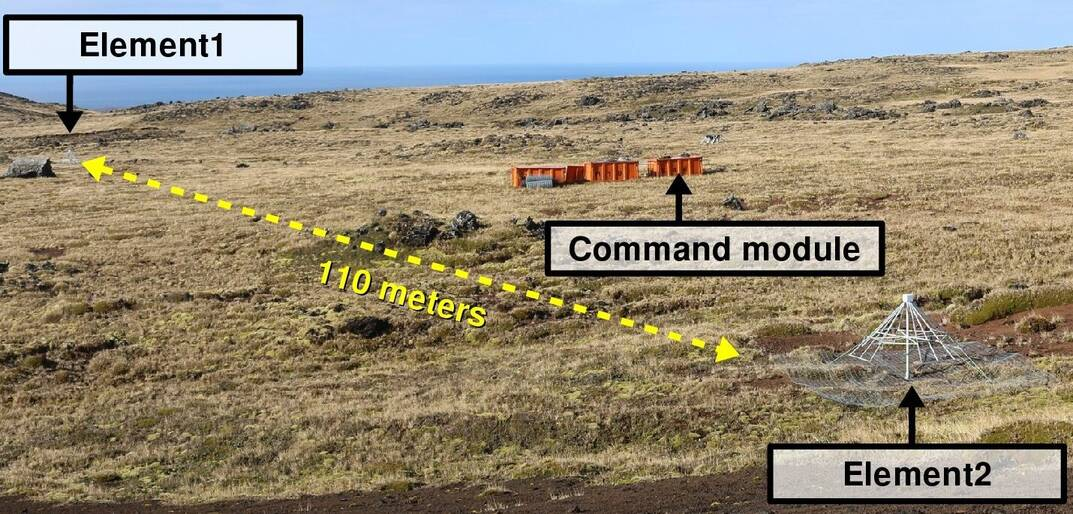
\includegraphics[width=\linewidth]{Figures/Albatros}
	\caption{The two-element, directly correlated \albatros\ pathfinder installed at the \prizm\ site. The pathfinder comprises two dual-polarization antennas separated by roughly 110 m on an east-west baseline. Coaxial cables connect the antennas to an orange shipping container that houses the readout electronics and serves as the "command module".}
	\label{Fig:albatros2}
\end{figure}

\section{Pathfinder System Signal Chain}

\begin{figure}
	\begin{center} 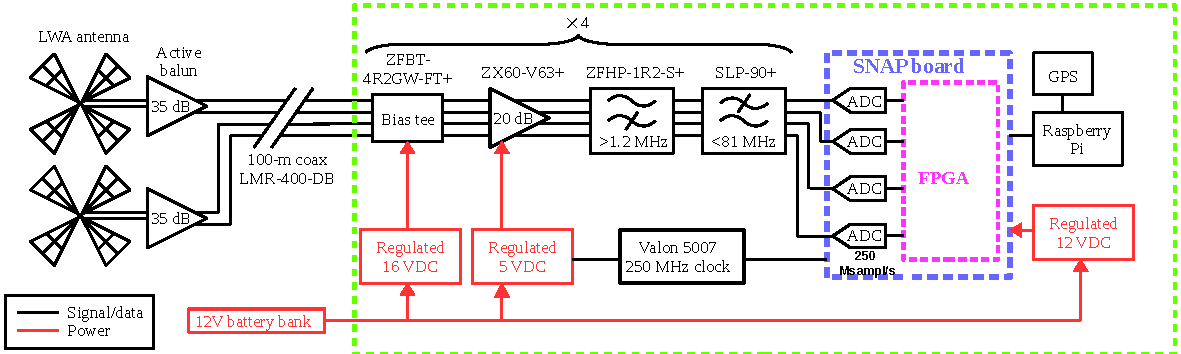
\includegraphics[width=\linewidth]{Figures/pathfinder_schematic.pdf}
		\caption{The pathfinder's two-element \albatros\ block diagram.  The signals from two dual-polarization LWA antennas~\citep{2012PASP..124.1090H} are amplified by front-end active baluns. The 100-m coaxial cables connect the SSE housed in a Faraday cage denoted by a green dashed box, with the antennas. A second-stage electronics chain is moved to each of the four antenna outputs. It consisting of filters and further amplification. A SNAP module comprises an on-board FPGA that calculates auto- and cross-spectra at 250~Msamp/s from and between the four inputs and digitizes the signals. A SNAP board is controlled by the Raspberry Pi, and the data is saved.}
		\label{Fig:albatros2_schem}
	\end{center}
\end{figure}

\subsection{Antenna}\label{s:antenna}

The pathfinder uses two Long Wavelength Array (LWA) antennas configured as a two-element interferometric array. The two dual-polarization antennas are separated by $\sim$\SI{110}{\meter} on an east-west baseline. The LWA antennas were selected for this project because they are relatively simple and are omnidirectionally patterned. The other important factor is that the LWA antennas have a long development history and therefore are a natural off-the-shelf choice for initial measurements. The antennas possess low gain; therefore, the Galactic noise is limited by a factor of 10 at a frequency range of \SIrange{30}{90}{\mega \hertz}~\citep{Memo28, Memo27}. Figure~\ref{Fig:LWA_mesh_gain} shows the gain in the zenith direction as a function of frequency. It also gives the realized gain (same direction), showing how the antenna is quite lossy at the lowest frequencies. Realized gain also takes into account the losses on the antenna. Due to the antenna being electrically short at the lowest frequencies, impedance mismatch losses are high. As a result, the realized gain curve is \SI{50}{\decibel} lower. The dB scale emphasizes how low gain/low efficiency the antenna is outside of its nominal operating range. The entire antenna and supporting structure sits on top of a ground screen that is roughly \SI{3}{\meter} on a side and is made of welded wire mesh. To prevent loss by absorption into the ground and also to stabilize the system temperature by isolating the antenna from a variable (e.g., dry versus wet) ground conditions, a conducting \SI{3}{\meter} on a side ground screen is necessary~\citep{Memo157}.

\begin{figure}
	\centering
	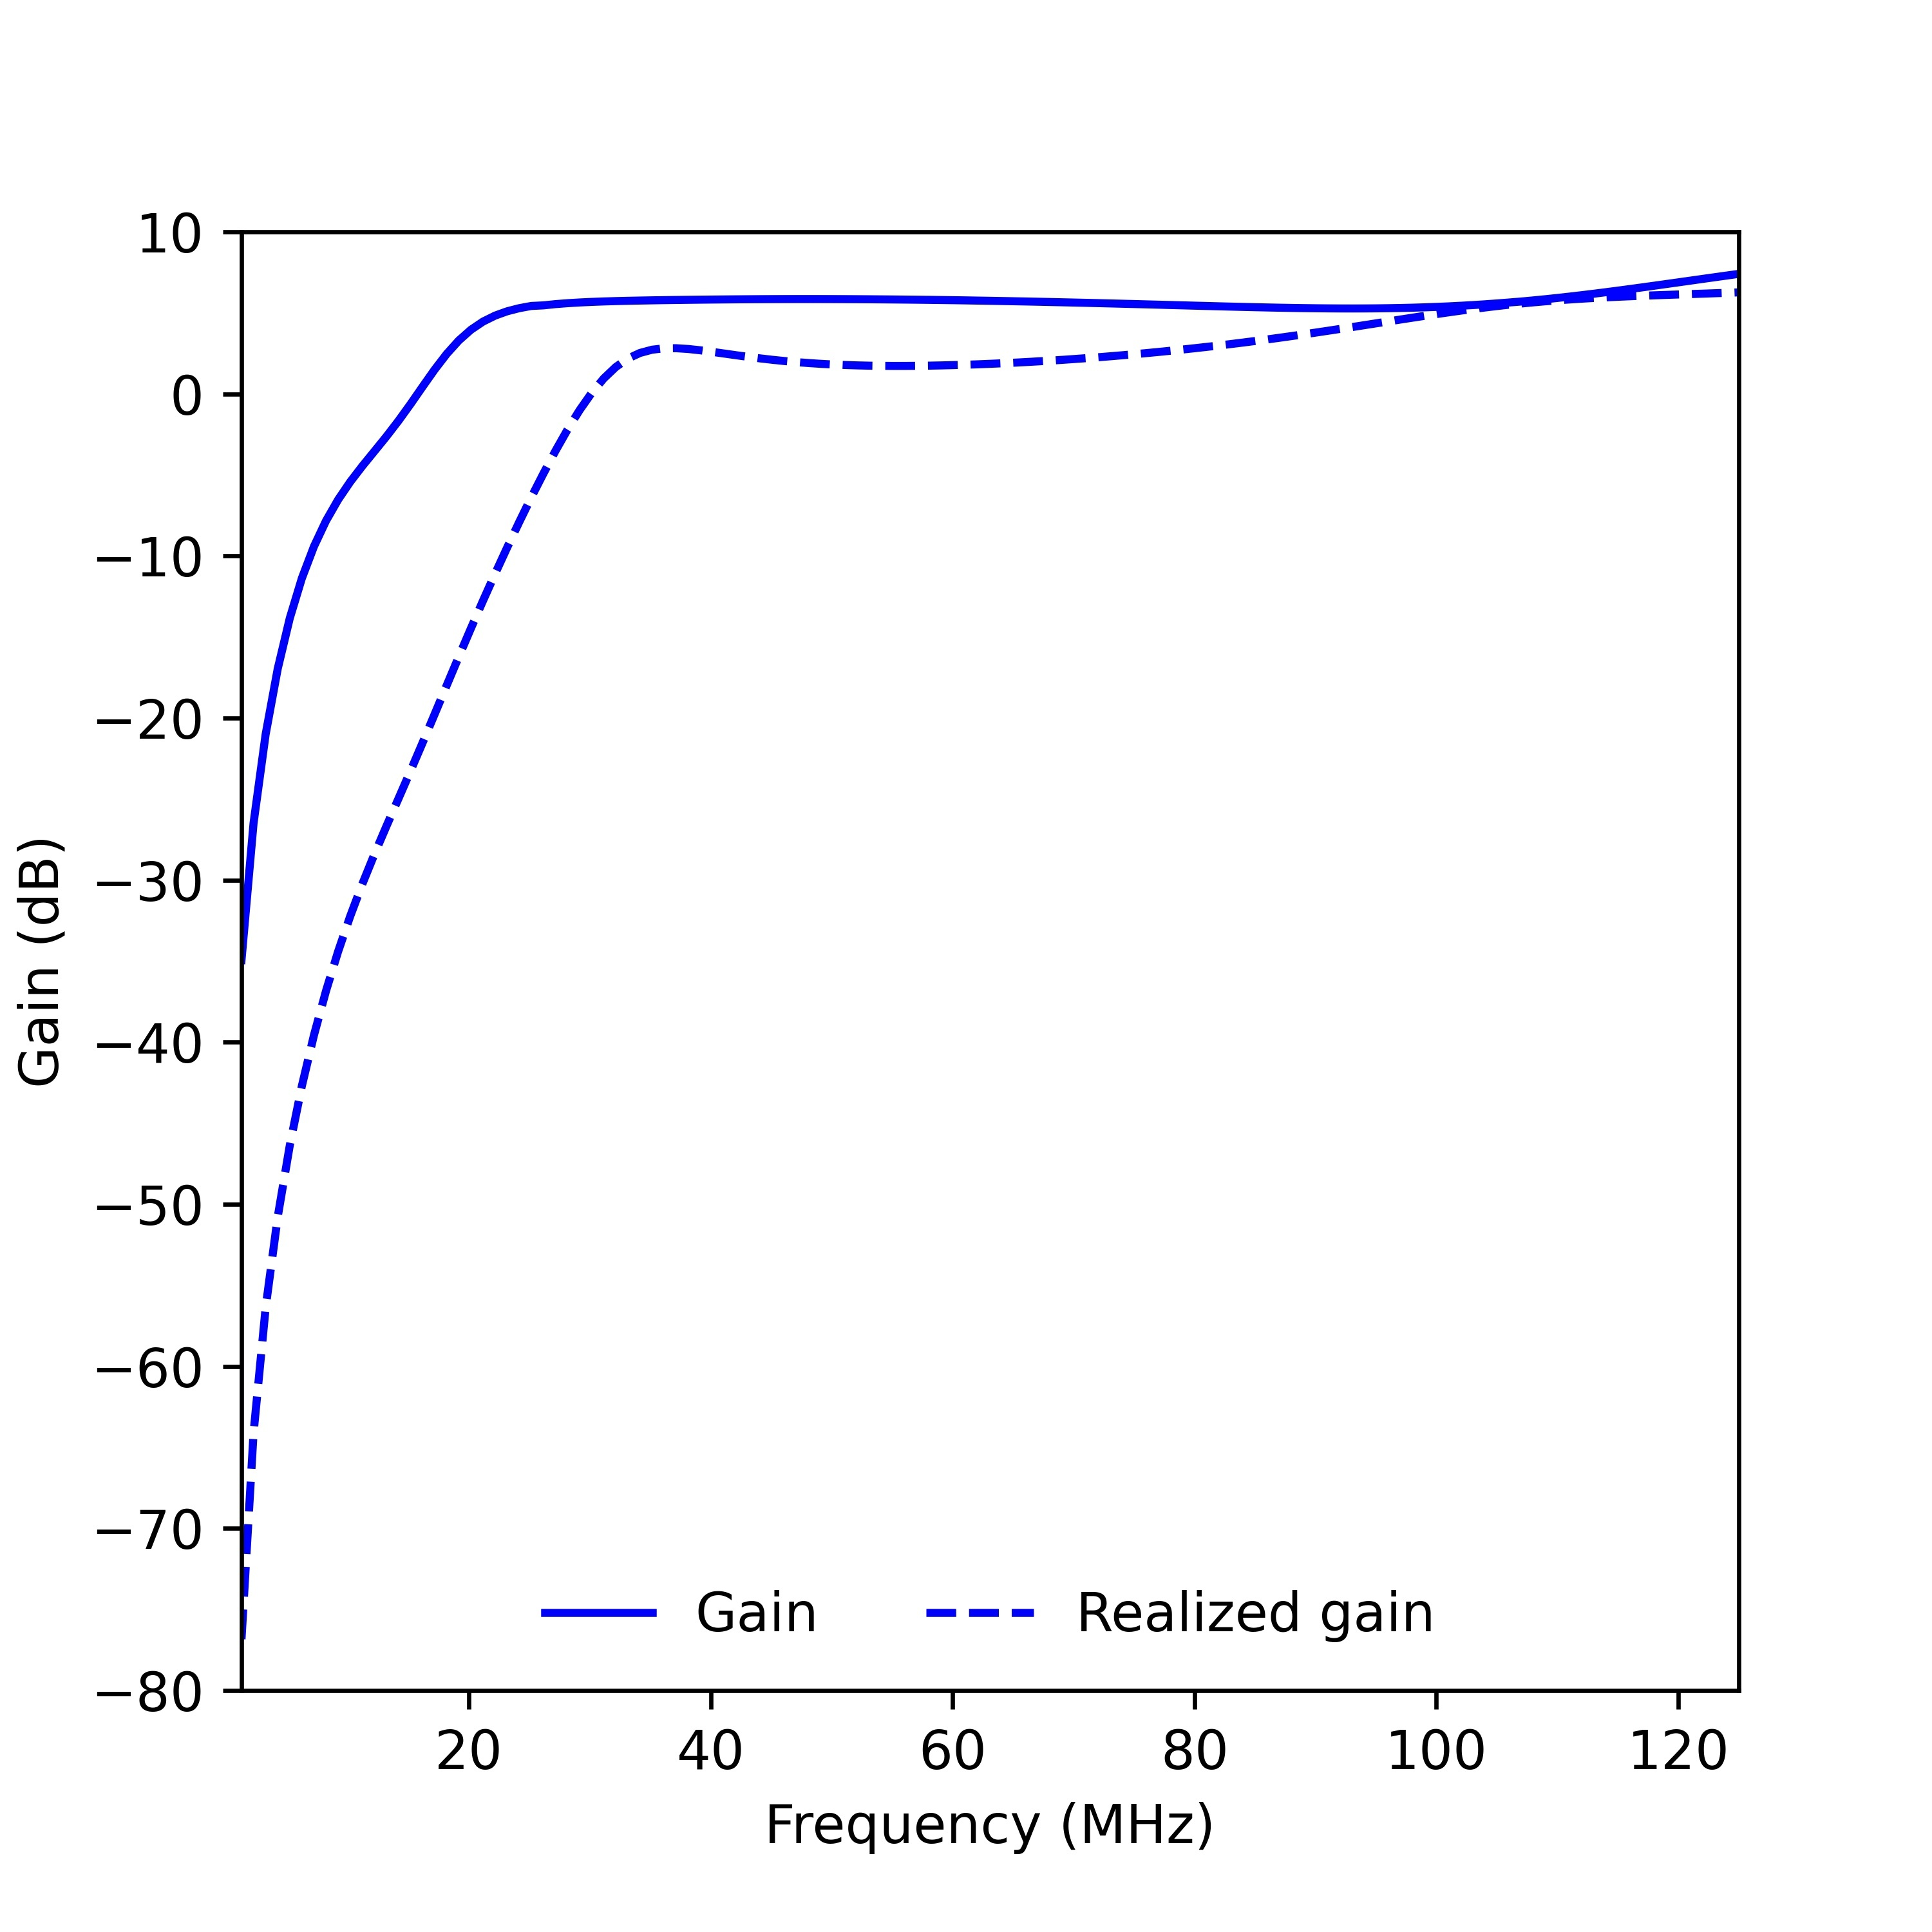
\includegraphics[width=0.7\linewidth]{Figures/LWA_mesh_gain}
	\caption{FEKO simulation for the antenna gain. The plot shows the gain in the zenith direction (which is always the peak gain) as a function of frequency; it also gives the realized gain (same direction), showing how the antenna is quite lossy. Due to the antenna being electrically short at the lowest frequencies, impedance mismatch losses are high. As a result, the realized gain curve is \SI{50}{\decibel} lower. Image credit: Tristan M\'ernard}
	\label{Fig:LWA_mesh_gain}
\end{figure}

\subsection{Front-end Electronics}\label{s:fee}

All the front end electronic (FEE) components are incorporated into a double-sided printed circuit board (PCB) as shown in Figure~\ref{Fig:balun} and the block diagram is shown in Figure~\ref{Fig:Balun Schematic}. One side of the PCB is a solid copper ground plane, and the other side is populated with components. The solid copper ground plane is aperiodically stitched to the grounded copper on the side populated with components. The active balun provides an input impedance of \SI{50}{\ohm} to each dipole. The Mini-Circuits GALI-74+ monolithic microwave integrated circuit (MMIC) amplifiers from both feed points amplify each signal by +24 dB of gain. A passive {180\degree} hybrid coupler differentiates the two GALI-74+ outputs. A low-pass filters the coupler output by \SI{150}{\mega\hertz} and gains \SI{12}{\decibel} from the Mini-Circuits GALI-6+ MMIC. The signal gets fed to a second amplifier. The output impedance of the FEE is matched to a \SI{50}{\ohm} \SI{100}{\meter} LMR400 coaxial cable having a nominal attenuation of $\sim$\SIrange{0.4}{3.7}{\decibel/100-m} at \SIrange{1.2}{81}{\mega\hertz}. The Mini-Circuits ZFBT-4R2GW-FT+ bias tee powers the FEE by \SI{16}{\volt} and extracts the RF signal by the use of the coaxial cable. The FEE has an overall gain of $\sim$ 36 dB and an overall noise figure of $\sim$ 2.7 dB to $\sim$ 2.9 dB~\citep{Memo35, 2012PASP..124.1090H}.

\begin{figure}
	\centering
	\begin{subfigure}[t]{0.52\textwidth}
		\centering
		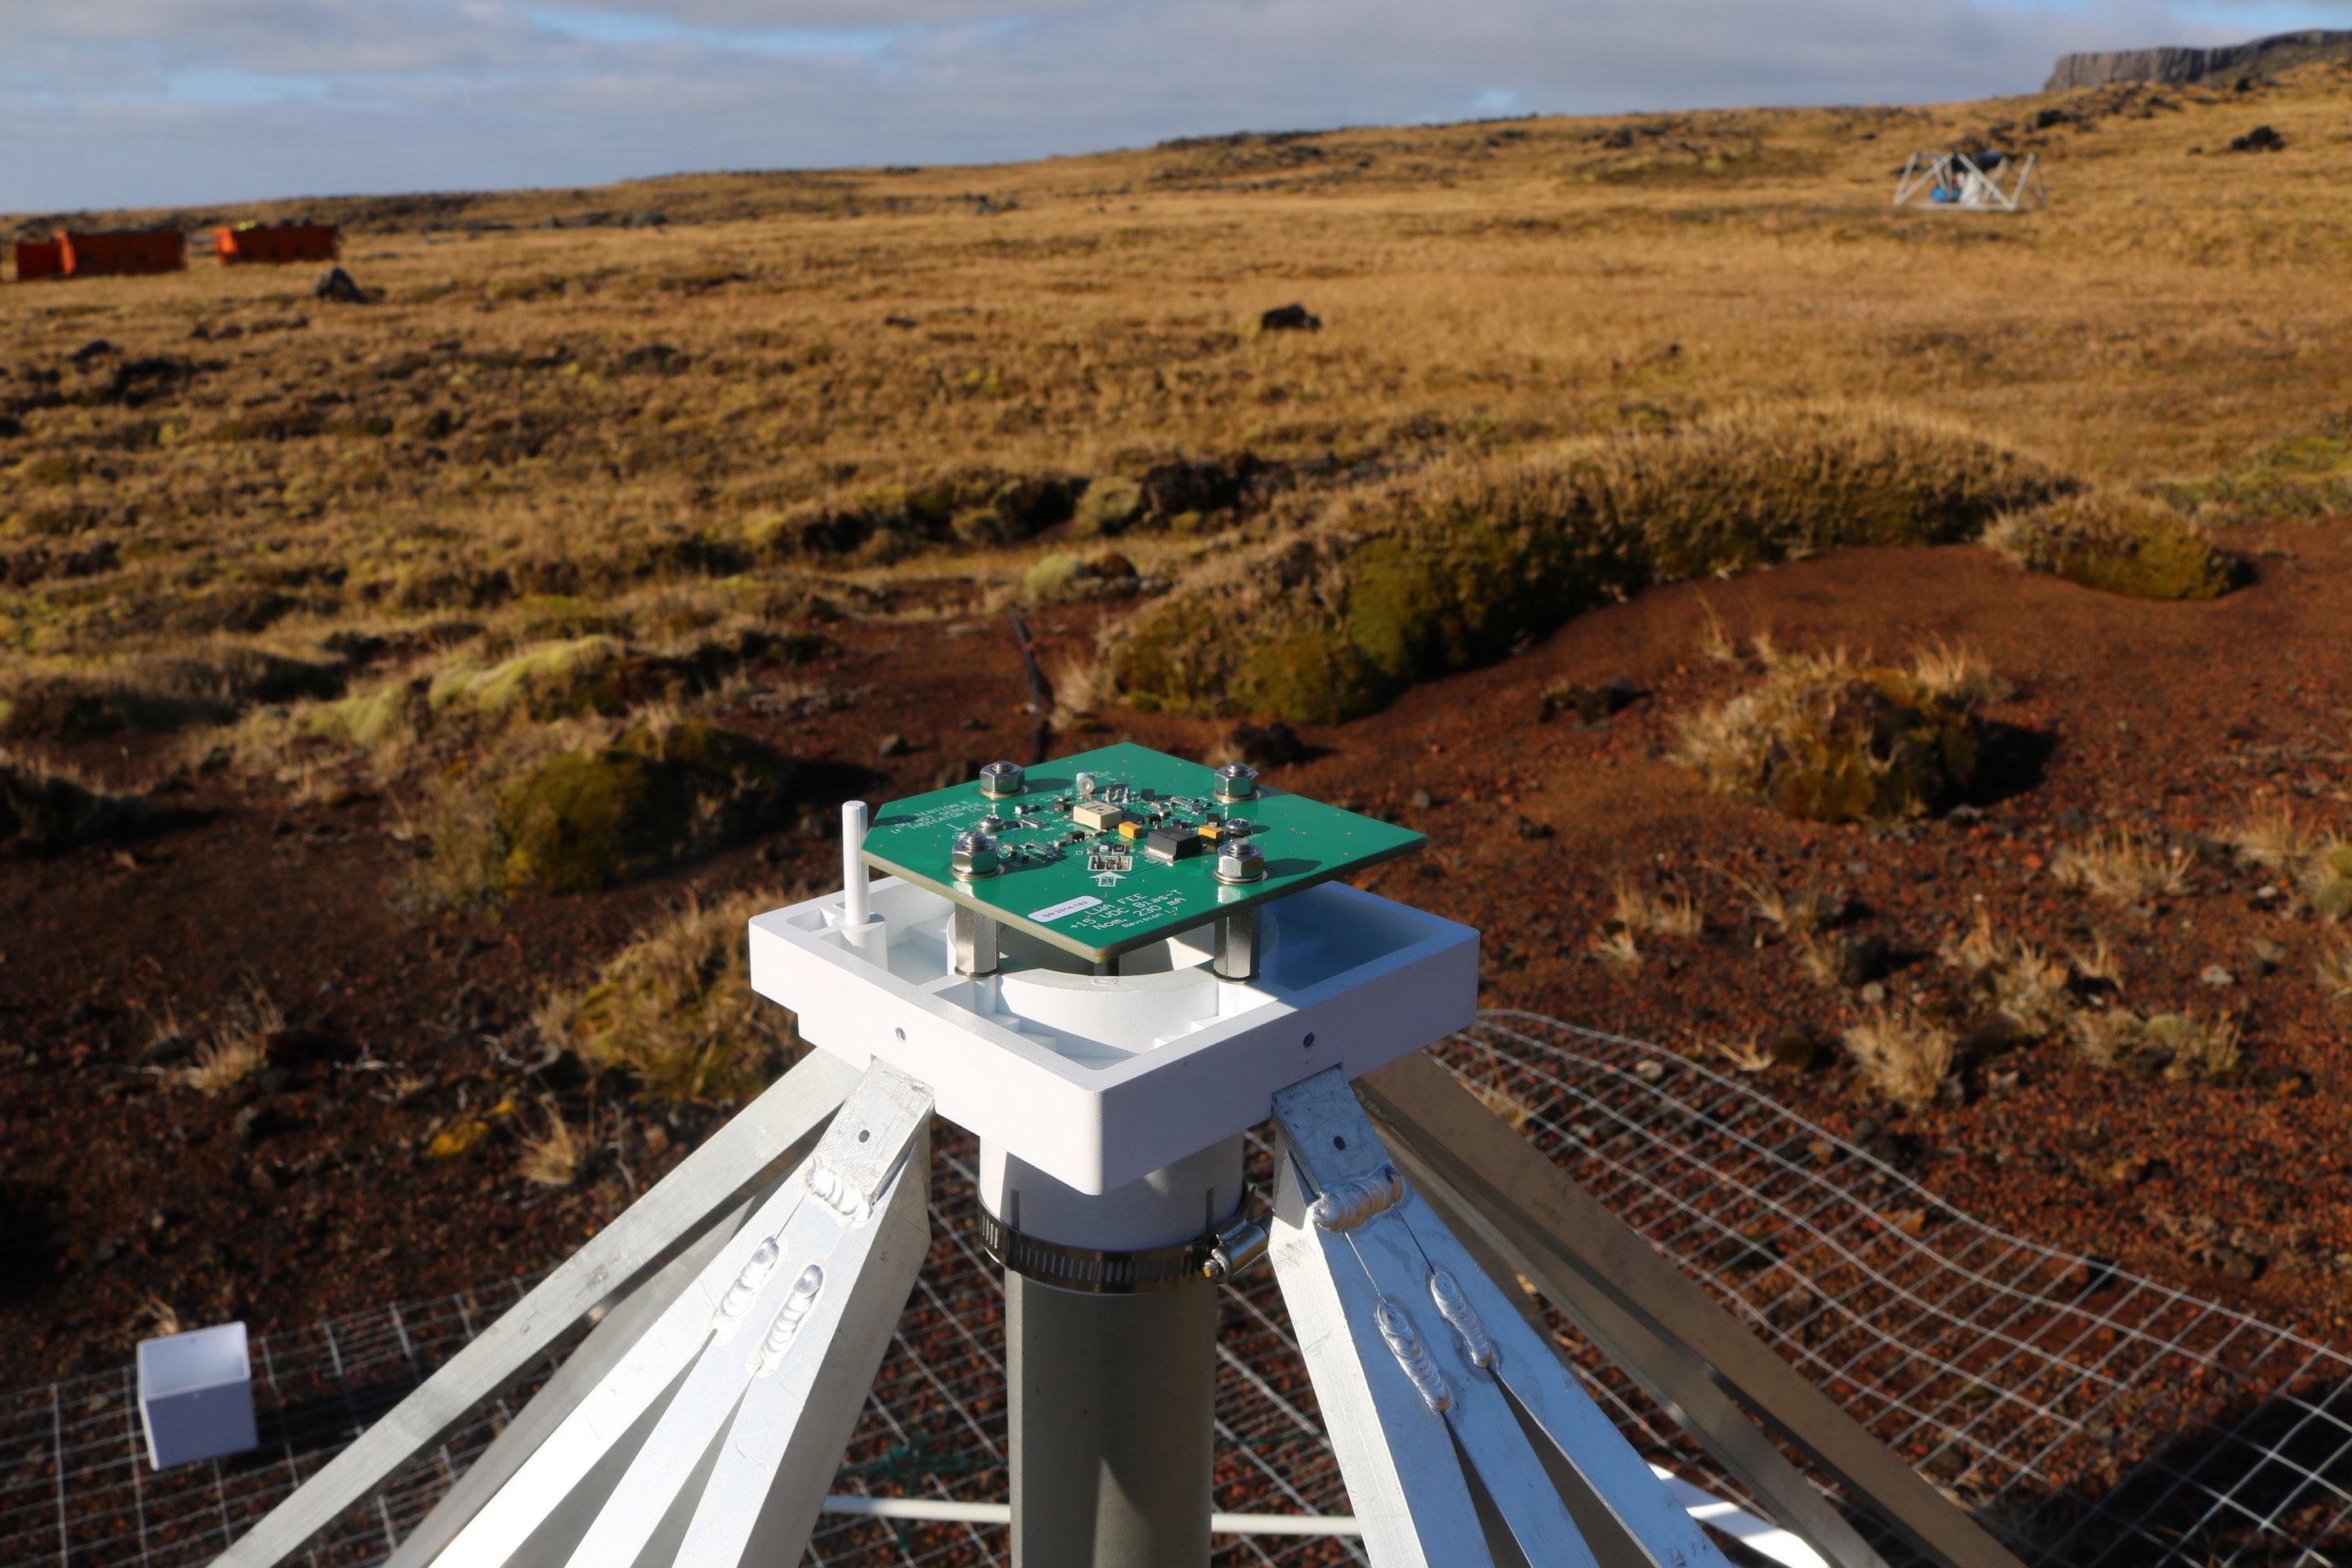
\includegraphics[width=\linewidth]{Figures/balun} 
		\caption{} \label{Fig:balun}
	\end{subfigure}
	\hfill
	\begin{subfigure}[t]{0.47\textwidth}
		\centering
		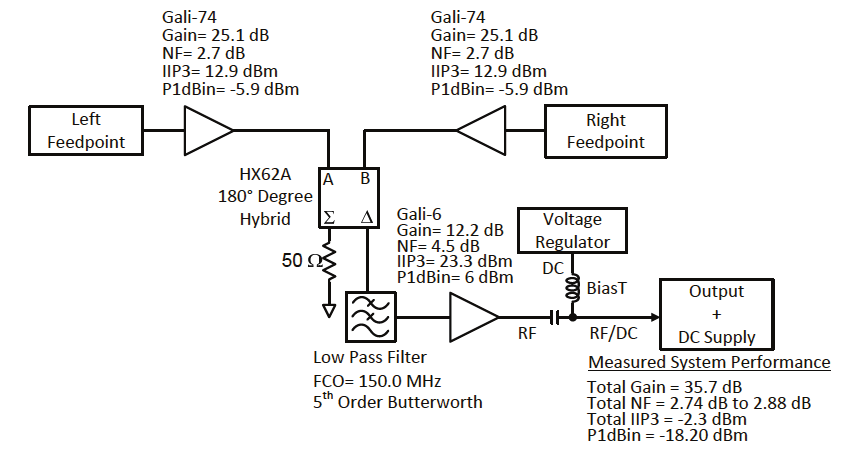
\includegraphics[width=\linewidth]{Figures/Balun_Block.png}
		\caption{} \label{Fig:Balun Schematic}
	\end{subfigure}
	\caption{{\bf (a)} Unenclosed FEE mounted on the pathfinder antenna supporting structure with the electronic components visible on the top part of the PCB. {\bf (b)} One polarisation block diagram of the FEE~\citep{2012PASP..124.1090H}} \label{Fig:fee}
\end{figure}

\subsection{Back-end Electronics}

The back-end electronics are housed in the Faraday cage shown in Figure~\ref{Fig:47093126504_fa0061a85b_o} and denoted by the green dotted line box in Figure~\ref{Fig:albatros2_schem}. The analog signal chain consists of a Mini-Circuits ZX60-V63+ amplifier with a \SI{20}{\decibel} gain, and a set of high- and low-pass filters (Mini-Circuits ZFHP-1R2+ and SLP-90+) that together band-limits the signal to \SIrange{1.2}{81}{\mega\hertz}. The amplifier operates at a frequency range of \SI{50}{\mega\hertz} - \SI{6}{\giga\hertz} and has a noise figure of $\sim$ 3.6 dB at its lowest operating frequency of \SI{\sim 50}{MHz}. The high- and low-pass filters present a nominal insertion loss of 0.2 dB and 0.14 dB at the center frequency of \SI{\sim10}{MHz}, respectively. AWR design environment simulation and analysis were used as shown in Figure~\ref{Fig:path} to plot the combined transfer function of the analog chain. The plot combines the S21 magnitudes in~dB of the low pass filter, high pass filter, and amplifier. It clearly shows that the cutoff frequency is \SI{\sim 90}{MHz} corresponding to the \SI{\sim 20}{\decibel} magnitude in dB.

\begin{figure}
	\centering
	\begin{subfigure}[t]{0.52\textwidth}
		\centering
		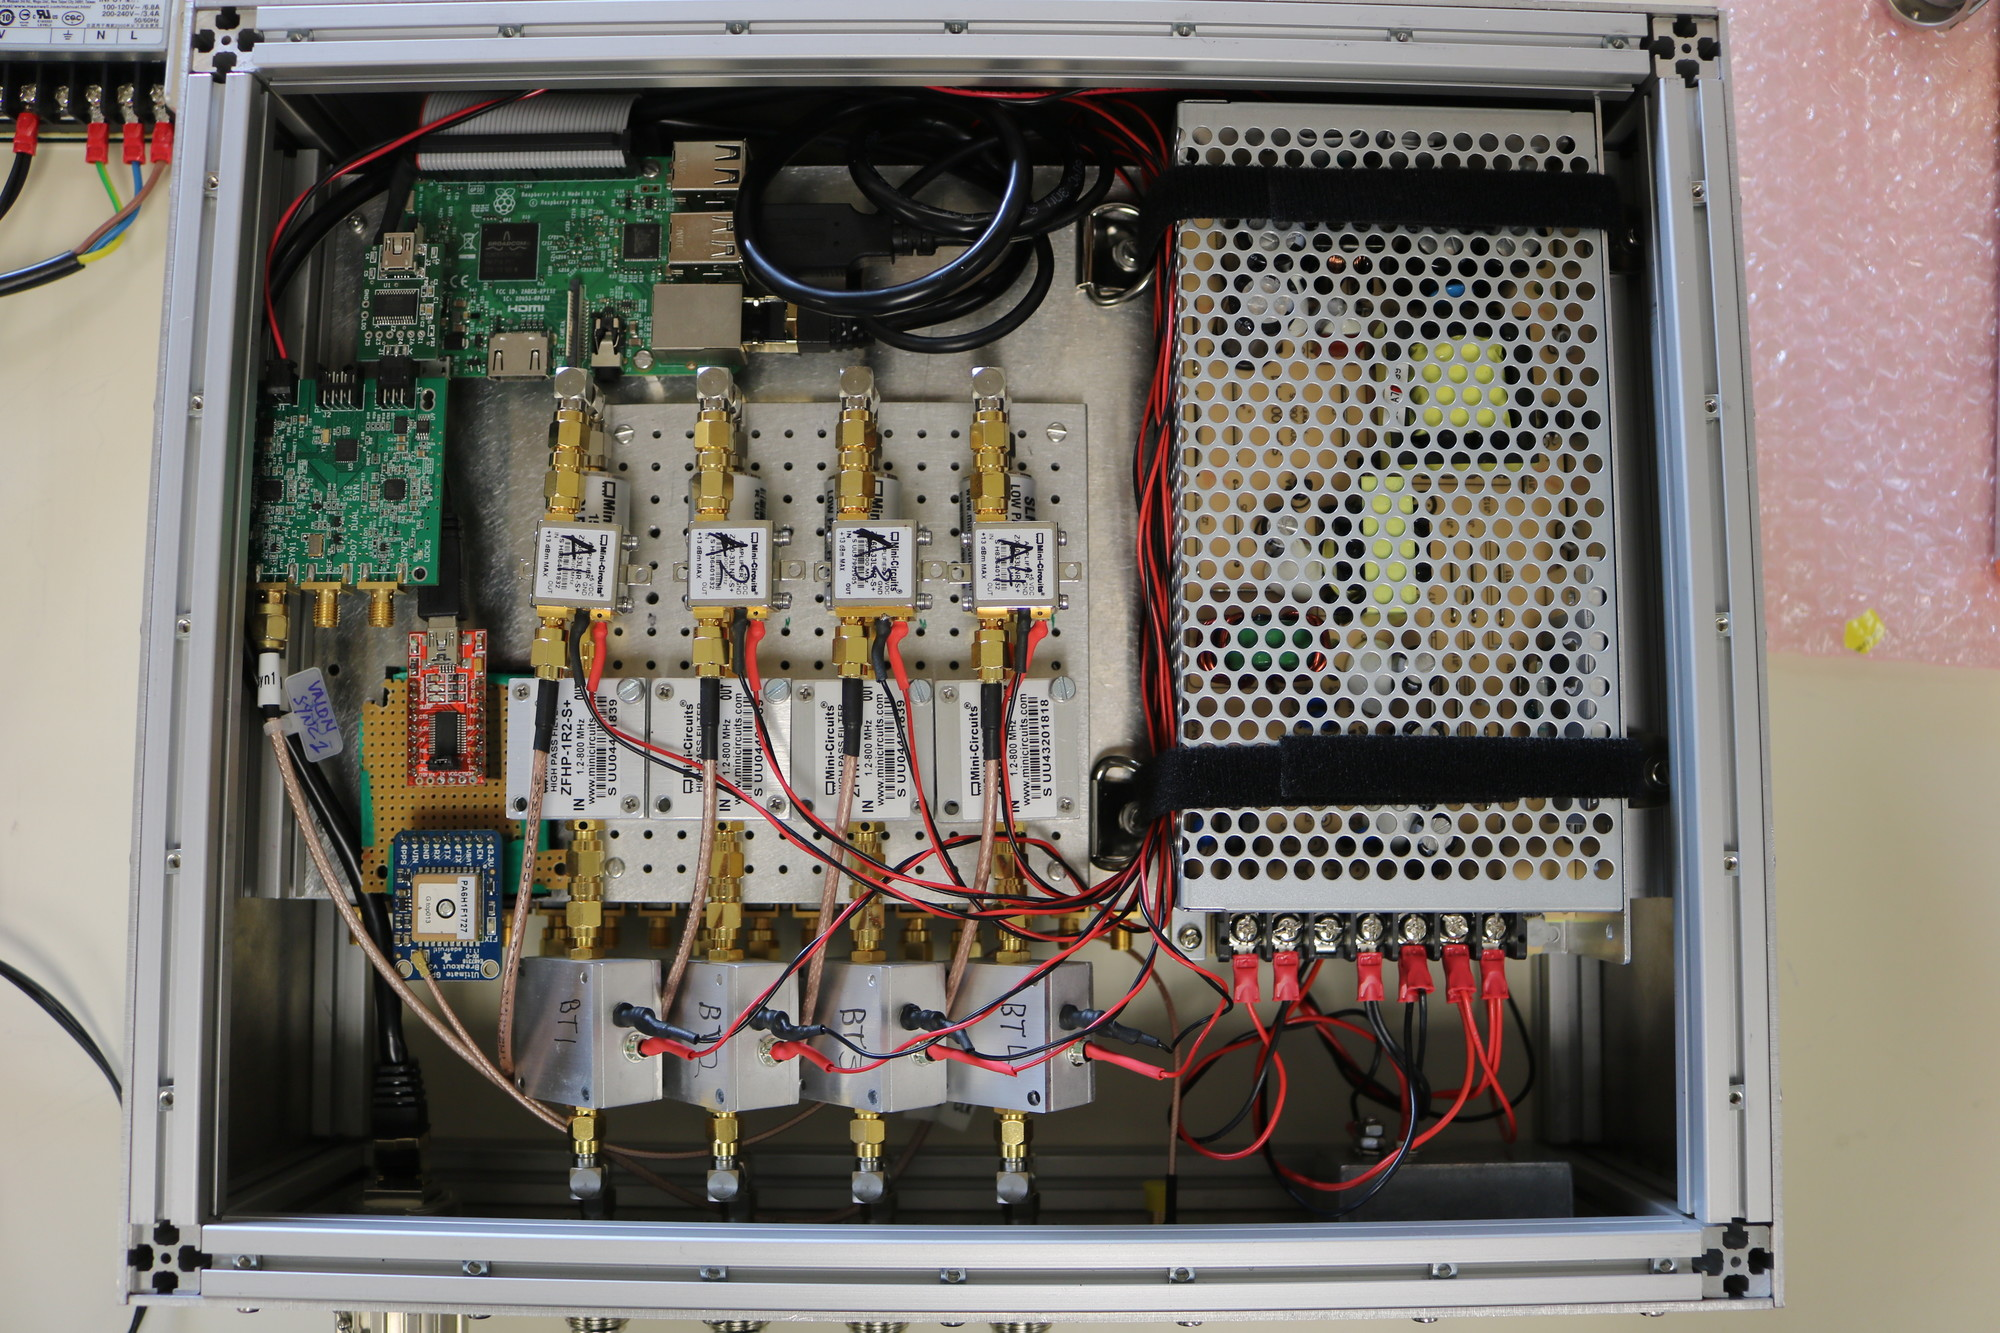
\includegraphics[width=\linewidth]{Figures/47093126504_fa0061a85b_o} 
		\caption{} \label{Fig:47093126504_fa0061a85b_o}
	\end{subfigure}
	\hfill
	\begin{subfigure}[t]{0.47\textwidth}
		\centering
		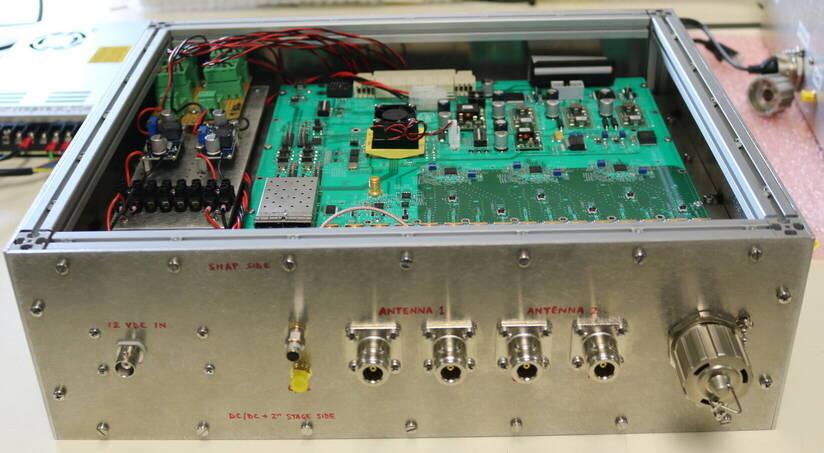
\includegraphics[width=\linewidth]{Figures/47093128324_04792aa5c5_o}
		\caption{} \label{Fig:47093128324_04792aa5c5_o}
	\end{subfigure}
	\caption{{\bf (a)} \albatros\ back-end electronics housed in the Faraday cage. The box mounts all components back-to-back on a central shelf so that everything can be accessed by opening opposing sides. One side of the mounting plate shows the amplifiers, pair of high- and low-pass filters, bias-tees, Valon 5007 frequency synthesizer module, RPi and Adafruit Ultimate GPS module. Component not visible on this side are mounted on the other side of the mounting plate. {\bf (b)} The bottom side of the \albatros\ Faraday cage, showing the mounted SNAP board and the regulatory circuit.} \label{Fig:faraday1}
\end{figure}

\begin{figure}
	\centering
	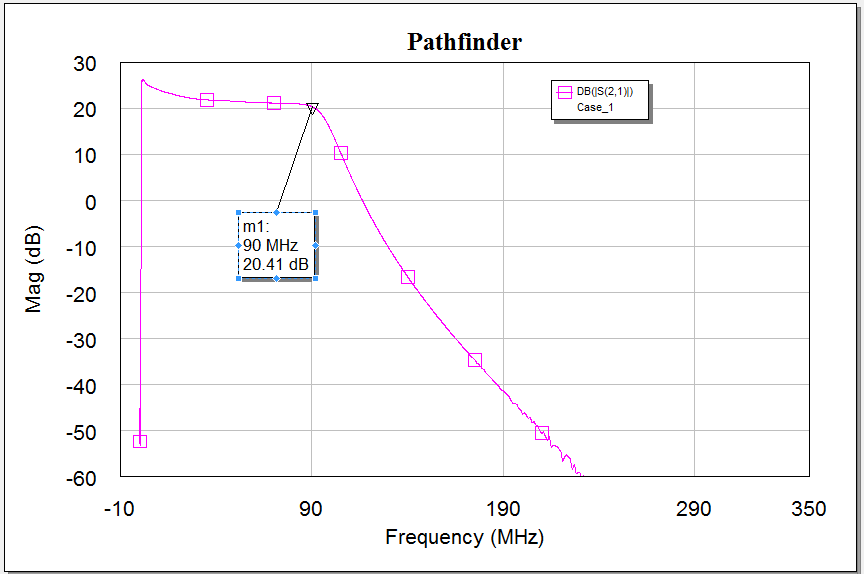
\includegraphics[width=0.7\linewidth]{Figures/pathfinder.PNG}
	\caption{A combined transfer function of the analog chain. The plot is a combination of the S21 magnitudes in~dB of the low pass filter, high pass filter and the amplifier. The cutoff frequency is at \SI{\sim 90}{MHz}.}
	\label{Fig:path}
\end{figure}

A Smart Network ADC Processor~\citep[SNAP;][]{2016JAI.....541001H} mounted in the Faraday cage in Figure~\ref{Fig:47093128324_04792aa5c5_o} samples incoming signals at \SI{250}{Msamp/s} using internal analog to digital converters (ADCs), with a clock signal provided by a Valon 5007 frequency synthesizer module. A frequency range between \SIrange{0}{125}{\mega\hertz} containing 2048 channels is created by the SNAP board, which also includes the on-board Xilinx Kintex~7\footnote{\url{http://www.xilinx.com/products/silicon-devices/fpga/kintex-7.html}}. The FPGA is programmed with spectrometer firmware that channelizes the ADC data and computes auto- and cross-spectra. The SNAP board is controlled by a Raspberry Pi (RPi), and the data rate of the average spectrum is about 400 MB/day (with compression), and this low volume allows the spectra to be stored on the RPi on-board SD card. The RPi absolute timing is provided by Adafruit Ultimate GPS module\footnote{\url{https://www.adafruit.com/product/746}}, connected to an active external GPS antenna.

\subsection{Power}
The two-element pathfinder system is powered using four \SI{12}{\volt}, \SI{200}{\ampere\hour} batteries wired in parallel, and charging is performed manually using a Honda EU30is\footnote {\url{http://www.hondaenergy.com/generators/honda-eu30is.html}} generator and a fuel cache that is kept at the observing site. The main advantage of using a SNAP board is its low power consumption, which enables long-term battery-powered operation. The total system power draw is \SI{\sim45}{\watt} and the pathfinder system can operate without interruption for $\sim$1 week when the batteries are fully charged. Table~\ref{table:budget} shows a rough power budget of the pathfinder system, taking into consideration the dual polarization antennas. During observations, the batteries are connected to DC/DC converters powering the SNAP board, FEE, amplifiers, and the clock. The DC-DC converters are housed inside the Faraday cage and provide \SI{12}{\volt} stable voltage output distributed to the buck and boost converters. An output of \SI{16}{\volt} from the boost converter powers the FEEs via the coaxial cable using the bias tees, the SNAP board is powered directly from the DC-DC converters, the amplifiers are powered by \SI{5}{\volt} from the buck converter.

\begin{table}
	\centering
	\begin{tabular}{|c | c | c | c |} 
		\hline
		Module & Power Dissipation (W) &  Voltage (V) & Current (A)\\  
		\hline
		SNAP board & $\sim$30 & 12 & 2.5\\
		\hline
		FEE and Dual Pol & $\sim$8 & 16 & 0.48 \\
		\hline
		2nd Stage Amplifier & $\sim$0.7 & 5 & 0.14\\
		\hline
		5007 Frequency Synthesizer & $\sim$2 & 5 & 0.4\\
		\hline
		RPi & $\sim$12.5 & 5 & 2.5 \\
		\hline
		\textbf{Total} & $\sim$53.2 &  & $\sim$6 \\
		\hline
	\end{tabular}
	\caption{The two-element pathfinder system ratings. The figures shown are from the datasheets of the various components and considering that the antennas are dual-polarization antennas.}
	\label{table:budget}
\end{table}

\section{Overview of Autonomous Stations}\label{s:autonomous}

The final ALBATROS array will consist of ten autonomous antenna stations separated by maximum baseline lengths of \SI{\sim 20}{\kilo \meter} as shown in \autoref{Fig:marion_map}. There are eight remaining planned installation sites. The Hydro shack and the \prizm\ site already have infrastructure installed, and Katedraal will remain unused. The ten installation sites (existing and planned) for the ALBATROS array have a ring-like pattern that is appropriate for imaging and produces an FWHM synthesized beam of $7'$ at \SI{5}{\mega\hertz} as shown in Figure~\ref{Fig:marion_map_beam}. The array beam promises an improved ($>10$ times better) resolution over existing measurements to date. Thus far, the ALBATROS main goal will be to map Galactic foregrounds at high resolution at low frequencies, which is crucial before doing cosmological observations of the dark ages. 

In April 2019, I was part of the deployment team in Marion Island, and I am going to discuss in detail the tasks associated with \albatros\ that we managed to complete during the three-week relief voyage.  

\begin{figure}
	\centering
	\begin{subfigure}[t]{0.5\textwidth}
		\centering
		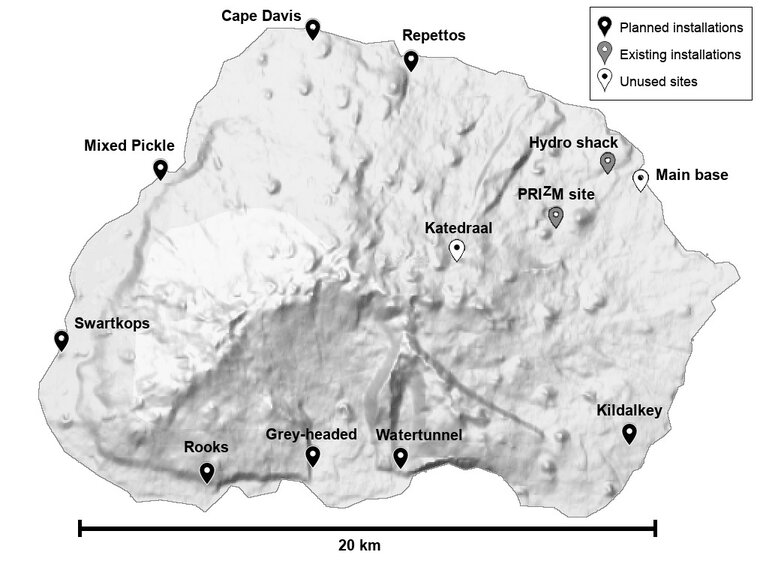
\includegraphics[width=\linewidth]{Figures/marion_map_annotated.jpg} 
		\caption{} \label{Fig:marion_map}
	\end{subfigure}
	\hfill
	\begin{subfigure}[t]{0.49\textwidth}
		\centering
		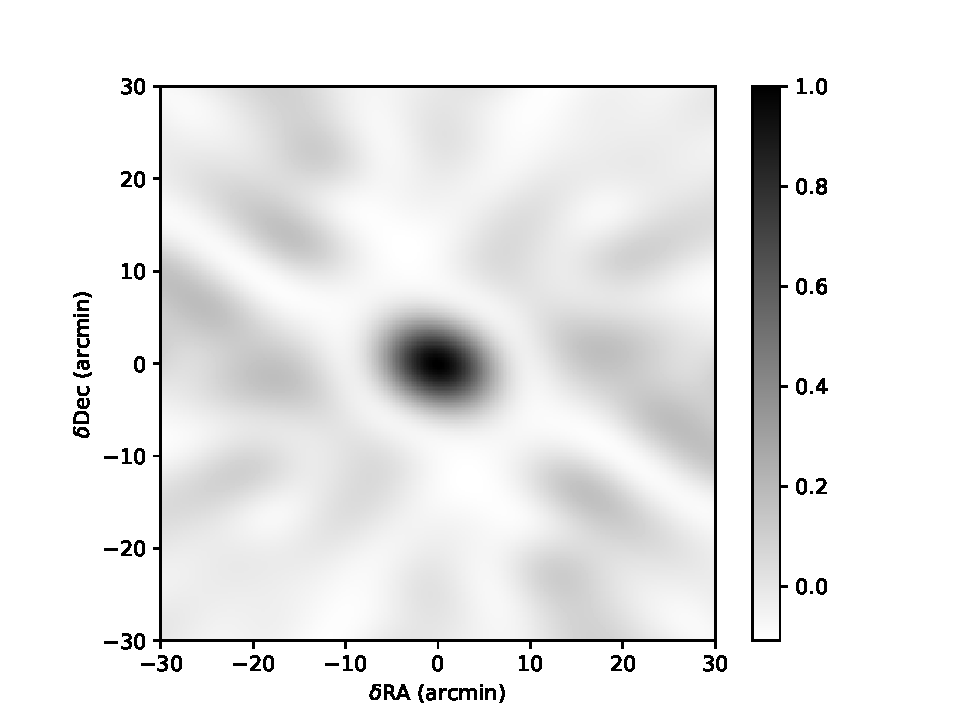
\includegraphics[width=\linewidth]{Figures/marion_beam_huts_2020}
		\caption{} \label{Fig:marion_beam}
	\end{subfigure}
	\caption{{\bf (a)} Map of Marion Island.  At present, the \albatros\ pathfinder antennas are located at the \prizm\ site and the hydro shack (gray markers). The black markers indicate the eight shore huts that will be used for potential installations of the \albatros\ antenna.  The white markers show the other infrastructure points available that will not be used for antennas. {\bf (b)} Synthesized beam at 5~MHz at zenith from the full \albatros\ array, using the existing and planned
		installation locations shown on the map.  A synthesized beam with a FWHM of $\sim7'$ is obtained using an octave of bandwidth spanning 3.5--7~MHz in a single snapshot.}
	\label{Fig:marion_map_beam}
\end{figure}

\section{2019 Marion Voyage}

The S. A. Agulhas II sails from Cape Town each year in April. The relief voyage preparations begin months before the ship sails; the team plans and makes decisions based on the next voyage's goals. One of the primary goals of the 2019 voyage was to install the prototype autonomous station.   The goal was to conduct an end-to-end system test under Marion's environmental conditions. The solar power budget, mechanical/electrical survival in wind and rain, and mouse proofing was the most critical considerations that were evaluated. The development and testing of improved designs and systems occur at the University of KwaZulu Natal radio astronomy lab. 

In preparation for the 2019 voyage, I designed and developed a prototype solar power supply system that paved the way for the solar power supply system installed in Marion Island as part of the autonomous stations. Figure~\ref{Fig:rooftop1} shows the solar panel used and the bin that enclosed the control electronics for the solar power system. Figure~\ref{Fig:rooftop2} shows the solar charge controller (Victron BlueSolar MPPT 75$\vert$15), \SI{12}{\volt} \SI{150}{\ampere \hour} battery, an Arduino that was used for logging the data from the solar charge controller to an SD card mounted in the RPi. 

\begin{figure}
	\centering
	\begin{subfigure}[t]{0.56\textwidth}
		\centering
		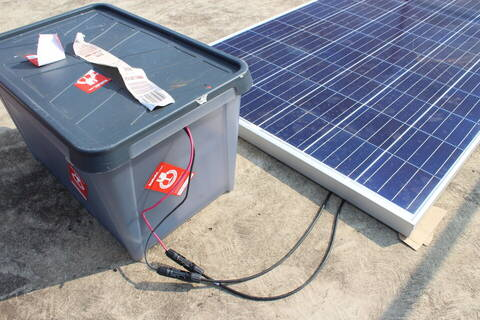
\includegraphics[width=\linewidth]{Figures/rooftop1} 
		\caption{} \label{Fig:rooftop1}
	\end{subfigure}
	\hfill
	\begin{subfigure}[t]{0.4\textwidth}
		\centering
		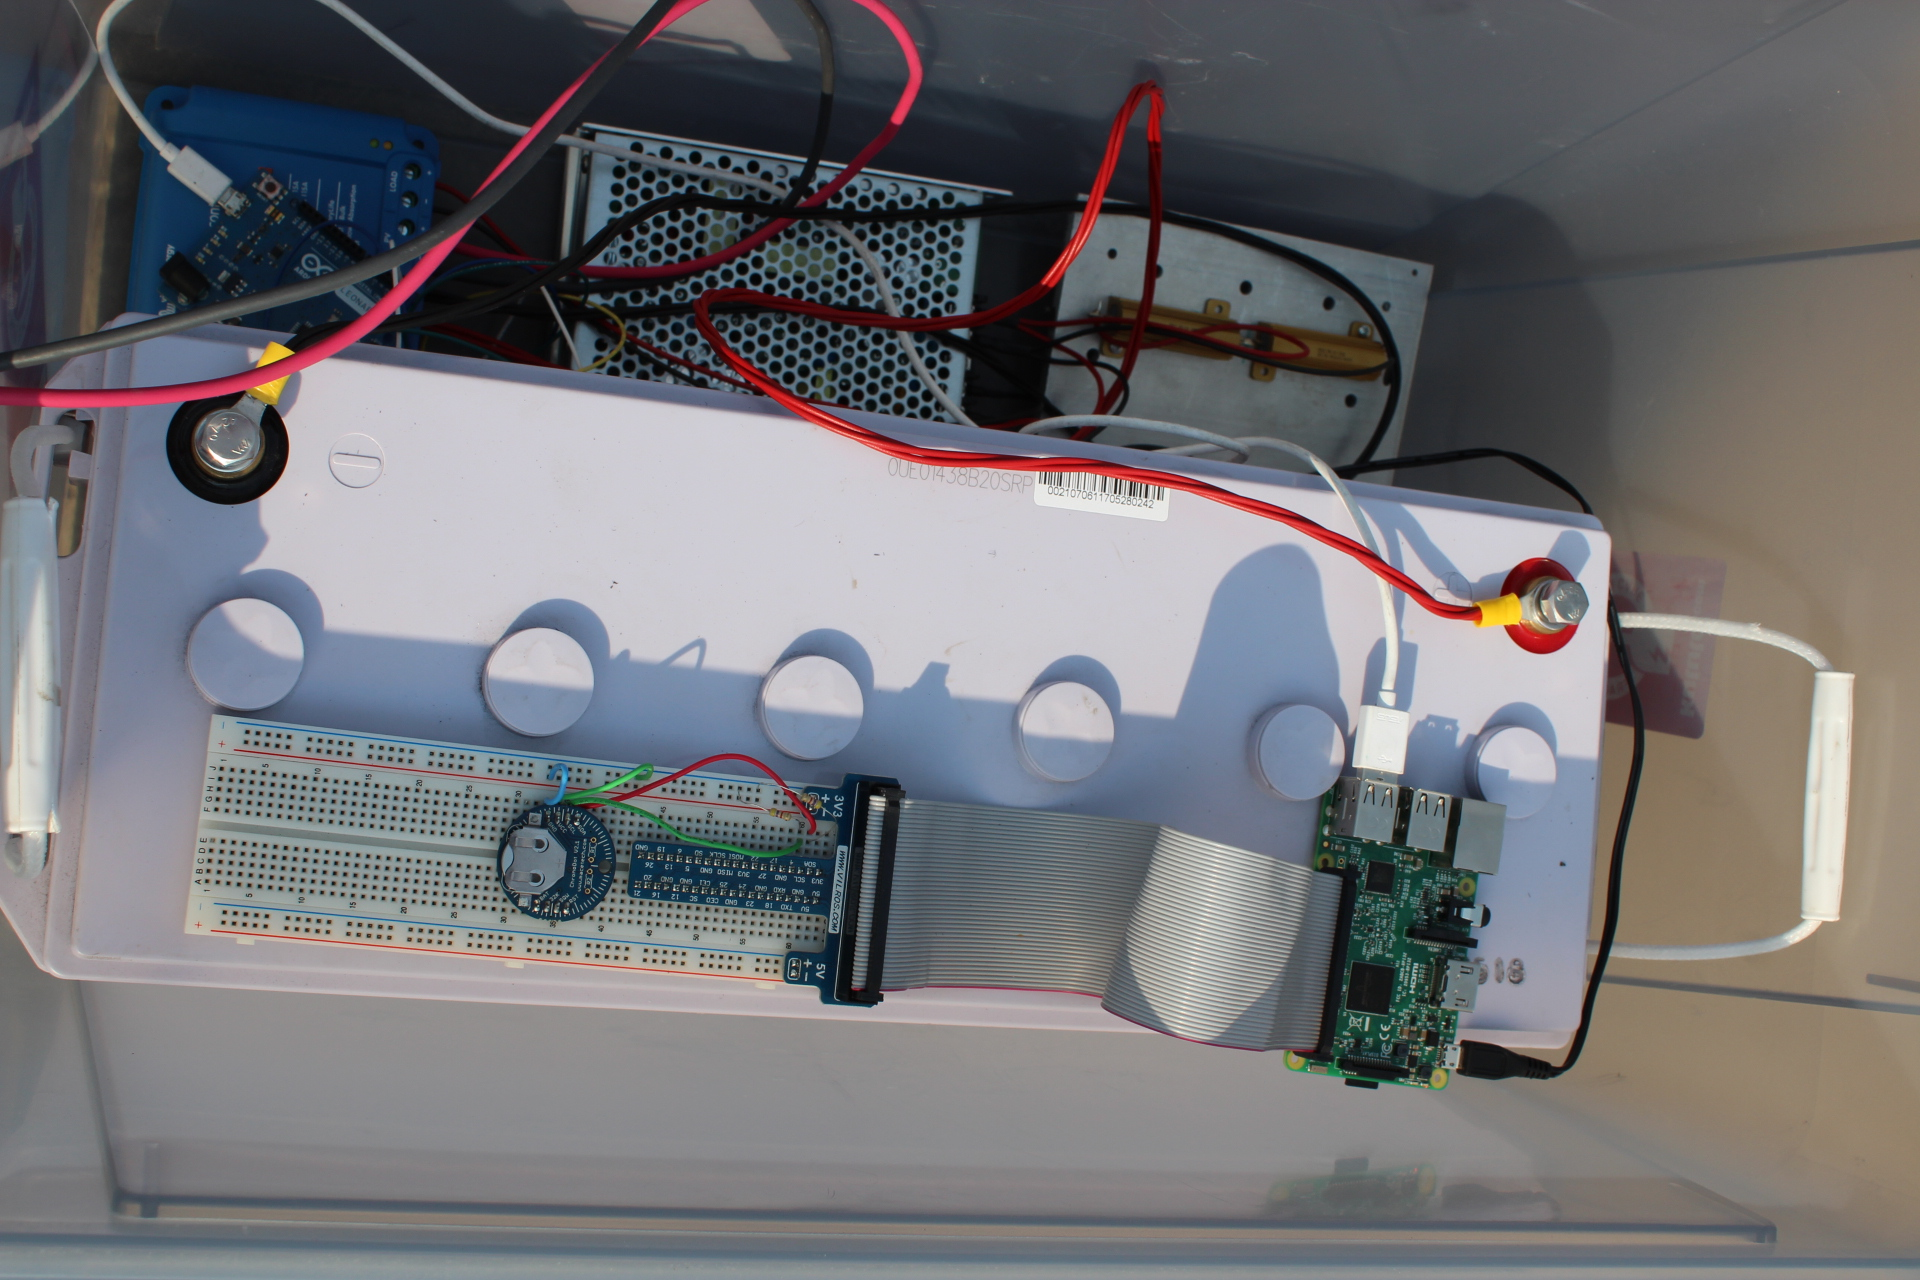
\includegraphics[width=\linewidth]{Figures/rooftop2}
		\caption{} \label{Fig:rooftop2}
	\end{subfigure}
	\caption{{\bf (a)} A prototype solar power supply setup. The prototype of the proposed system was tested on the roof of H Block at the UKZN. The solar panel which was used was the Enersol 300 and the control electronics are enclosed in the weather proof plastic bin. {\bf (b)} Interior of the enclosure. Inside the enclosure was the solar regulator which was monitored via a communication port, a single\SI{12}{\volt} \SI{150}{\ampere \hour} battery, an Arduino board which was programmed for serial to Universal Serial Bus (USB) communication, the Rpi which was connected to the sdr clock module for proper timing and syncronisation stored the data which was monitored from the solar regulator, the DC-DC converter regulated the voltage to the \SI{6}{\ohm} high power resistor.} 
	\label{Fig:History}
\end{figure}

Because of the weather conditions in Marion Island, the pathfinder system can shut down for an extended period without observations. A solar power supply system was selected because the \albatros\ stations are required to run continuously without manual intervention and charging. Therefore, the solar panels need to be appropriately sized, given the power budget and frequently overcast conditions. Also, interferometers are less susceptible to RFI that might be locally generated from the charge controllers and other switching components. Thus, a solar power system solution was implemented on the first autonomous station to run the system autonomously continuously. Total power experiments like \prizm\ are more susceptible to RFI; consequently, a manual charging method is used.   

During the relief voyage, the installation process included mechanical assembly and alignment of the antenna structure, laying coaxial cables, installing three solar panel mounts (with three panels each, for a total of nine panels), and installing a small processing hub consisting of a plastic bin housing the readout electronics, two batteries, and power control electronics. The first autonomous station signal chain shown in Figure~\ref{Fig:albatros1_schem} was installed in April 2019 at the hydroshack site (\ang{46;52.205;}S, \ang{37;50.612;}E) on Marion Island. The installation was the first step in testing the technologies required to create the full array. A similar antenna and front end active balun discussed in (\S\ref{s:antenna} and \S\ref{s:fee}) were used, and the back-end electronics and the power system are discussed in detail below.

\section{Autonomous Station Signal Chain}

\begin{figure}
	\begin{center}
		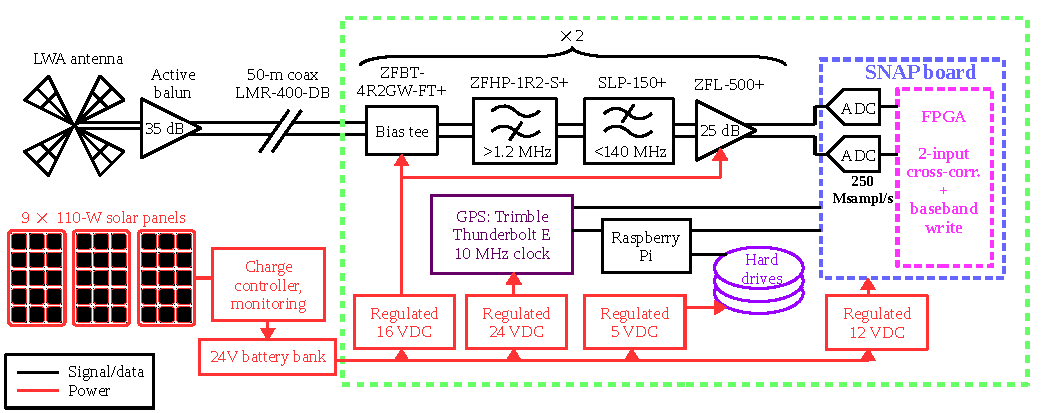
\includegraphics[width=\linewidth]{Figures/albatros_single_schematic}
		\caption{Single-antenna autonomous station block diagram. A dual-polarization LWA antenna, equipped with an active front-end balun, connects via a \SI{50}{\meter} coaxial cables to the back-end readout electronics and is housed in a Faraday cage green dashed box. Each of the two antenna signals is allowed to pass through a second-stage electronics chain consisting of filters and further amplification. A SNAP board includes an on-board FPGA that measures channelized baseband and spectra from both inputs and digitizes the signals at 250~Msamp/s. The SNAP board is controlled by a Raspberry Pi, and the baseband data and spectra are obtained. Baseband data are stored on the external hard drives. Solar panels charge a 24-V battery bank, which powers the system.}
		\label{Fig:albatros1_schem}
	\end{center}
\end{figure}

For the autonomous station, the same LWA antenna and FEE are used. The hydroshack site was assessed to avoid installing the hardware on top of a mire, and we were able to spot even terrain and were suitable for installing our hardware. The hydroshack site is a reasonable hiking distance from the main base, yet sufficiently far to reduce base-generated RFI.

\subsection{Back-end Electronics} 

\begin{figure}
	\centering
	\begin{subfigure}[t]{0.52\textwidth}
		\centering
		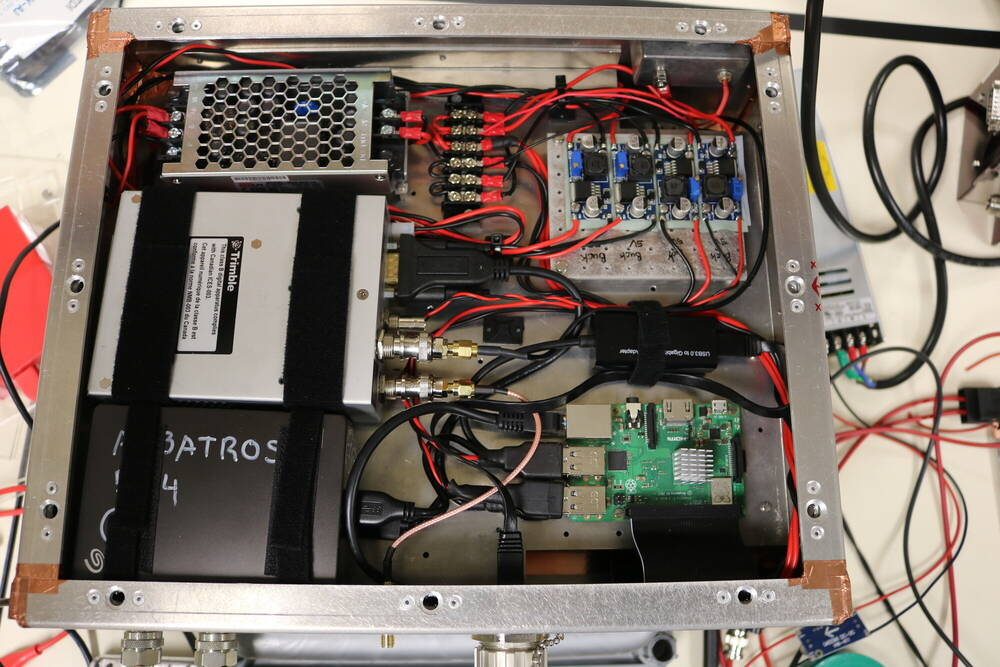
\includegraphics[width=\linewidth]{Figures/46966493985_44aa8ac326_o} 
		\caption{} \label{Fig:46966493985_44aa8ac326_o}
	\end{subfigure}
	\hfill
	\begin{subfigure}[t]{0.47\textwidth}
		\centering
		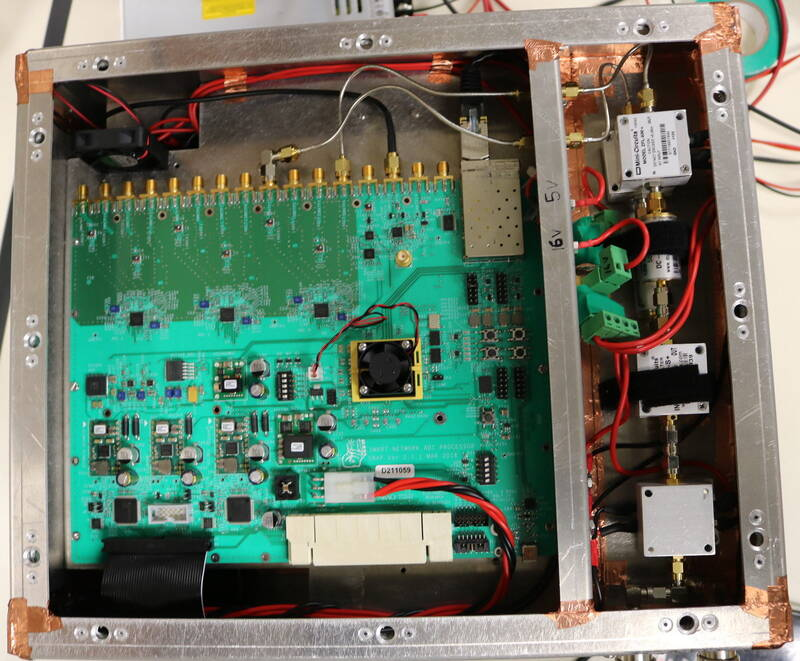
\includegraphics[width=\linewidth]{Figures/47882594521_3895effd86_o}
		\caption{} \label{Fig:47882594521_3895effd86_o}
	\end{subfigure}
	\caption{{\bf (a)} One side of the mounting plate with visible power distribution circuitry is shown in the single autonomous station Faraday cage, Trimble Thunderbolt E GPS-disciplined clock module, external hard drives and RPi. {\bf (b)} The analog signal chain mounted in the RF partition on the left and the SNAP board mounted on the right in the single autonomous station Faraday cage.} \label{Fig:faraday}
\end{figure}

The back-end electronics are very similar to those used for the 2-element pathfinder. However, a few key differences are external hard drives to store data and cross-correlate offline afterward and a Trimble Thunderbolt E GPS-disciplined clock module. Also, there were revisions done on the enclosure. The enclosure was a laser-cut, folded sheet metal design with captive quarter-turn fasteners to make it easier to assemble and more field-friendly.

The Faraday cage shown in Figure~\ref{Fig:46966493985_44aa8ac326_o} and denoted by the green dotted line box in Figure~\ref{Fig:albatros1_schem} is located \SI{50}{\meter} away from the antennas. The analog signal chain shown in Figure~\ref{Fig:47882594521_3895effd86_o} consists of a pair of high- and low-pass filters (Mini-Circuits ZFHP-1R2+ and SLP-150+) that together band-limit the signal to \SIrange{1.2}{140}{\mega\hertz}, and after the filters is the Mini-Circuits ZFL-500+ amplifier with a \SI{25}{\decibel} typical gain. The amplifier that I selected is the new change with respect to the 2-element pathfinder. The amplifier operates at a frequency range of \SIrange{0.05}{500}{\mega\hertz} which is well within our desired frequency range. An AWR simulation shown in Figure~\ref{Fig:auto} shows the plot of a combination of S21 magnitudes in~dB of the low pass filter, high pass filter, and the amplifier. It clearly shows that the cutoff frequency is \SI{\sim 150}{MHz} corresponding to the \SI{\sim 24}{\decibel} magnitude in dB. The autonomous station signal chain response is flatter with higher gain, as shown in Figure~\ref{Fig:comparison}.

\begin{figure}
	\centering
	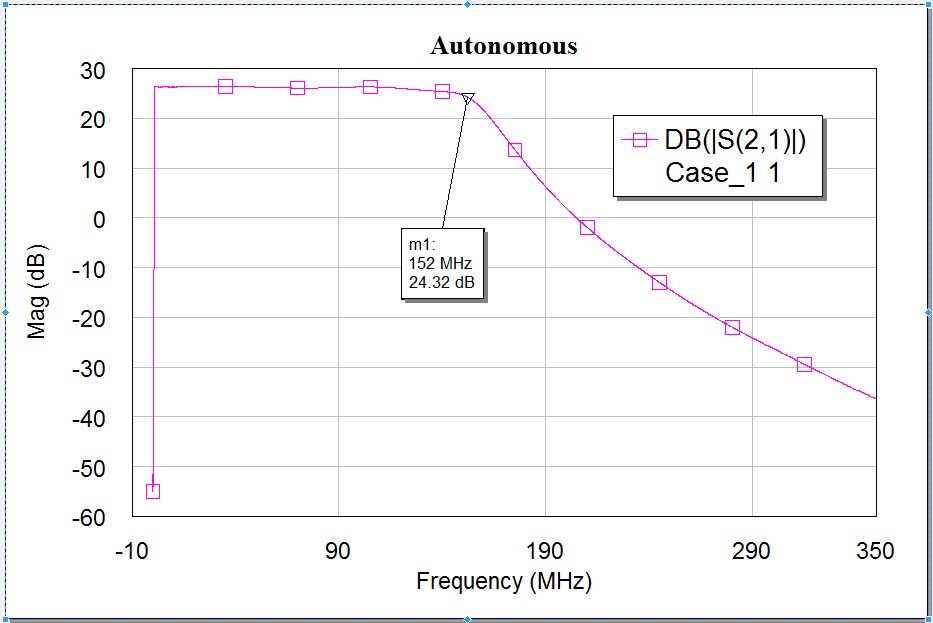
\includegraphics[width=0.7\linewidth]{Figures/auto}
	\caption{Autonomous station analog chain response. The plot is a combination of the S21 magnitudes in~dB of the low pass filter, high pass filter and the amplifier. It shows that the cutoff frequency is \SI{\sim 150}{MHz} corresponding to the \SI{\sim 24}{\decibel} magnitude in dB.}
	\label{Fig:auto}
\end{figure}

\begin{figure}
	\centering
	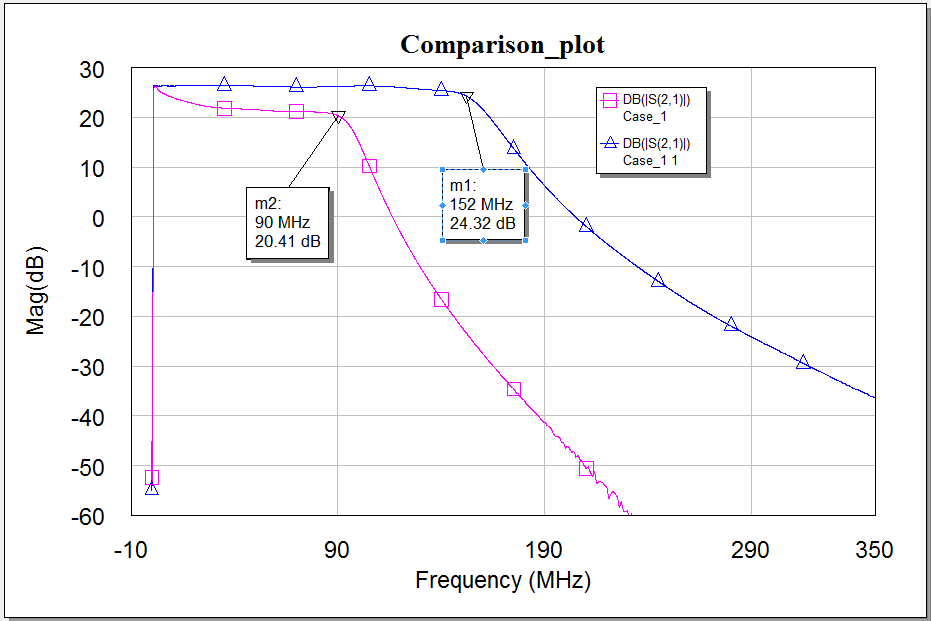
\includegraphics[width=0.7\linewidth]{Figures/comparison}
	\caption{The comparison of the pathfinder and autonomous station analog chain response. The autonomous station signal chain response in blue is flatter with higher gain compared to the pathfinder response in pink.}
	\label{Fig:comparison}
\end{figure}

In comparison to the two-element pathfinder, the cut-off frequency of the low-pass filter increased from \SIrange{81}{140}{\mega\hertz} to capture downlink signals at \SIrange{137}{138}{\mega\hertz} from the ORBCOMM satellite constellation. The ORBCOMM signals are beneficial to the final \albatros\ array because they provide a convenient means for synchronization across the antenna stations, serving as a backup to the GPS timing discussed below. Actual lab tests recommend that on time scales of \SI{\sim 30}{\second}, relative timing between various autonomous stations can be estimated to a precision of better than a couple of tenths of a nanosecond utilizing a solitary satellite. At \SI{10}{\mega\hertz} the correlation phase error is $\lesssim1^\circ$. With open-access orbits and various satellites commonly within the field of view, the ORBCOMM baseband data supposedly saved simultaneously with the astronomical data can provide offline synchronization of the ALBATROS stations. Since the ORBCOMM and science data are recorded simultaneously by the same system, enhancement to the timing calibration can be applied in post-processing.

The signals are then digitized at \SI{250}{Msampl/s} by the SNAP board mounted in the Faraday cage in Figure~\ref{Fig:47882594521_3895effd86_o}. A Trimble Thunderbolt E GPS-disciplined clock module creates a \SI{10}{\mega\hertz} reference that is locked from the SNAP board internal ADCs. The reason for phasing out a Valon was because of its wide frequency band and having limited applications. A Trimble Thunderbolt E GPS-disciplined clock module replaced the Valon for high volume synchronization applications. The SNAP board FPGA processes channelized baseband data for every polarization over tunable frequency windows inside the \SIrange{0}{125}{\mega\hertz} range, with the options of 1-, 2-, 4-bit baseband channelization, and auto-and cross-spectra from the two polarizations over the full \SIrange{0}{125}{\mega\hertz} range, collected more than few-second spans. As we are doing long term observations, 1-bit channelization enables us to store data without running entirely out of external hard drive space. However, the auto spectrum information cannot be recovered from 1-bit data. The appropriate transition levels must be tuned/set for 2- and 4-bit quantization. Hence, the higher the number of bits, the higher the signal fidelity and the higher volumes of data.

The decrease in bit profundity happens simply after the SNAP board has channelized the baseband, and the cross-channel spillage (due to, e.g., RFI and inclines in RF power as observed by the ADCs) is this way unaffected by the low bit profundity. A polyphase filter bank (PFB) is used in the FPGA firmware to do the channelization. The incoming analog signal passes through a polyphase filter bank after being sampled by the ADC. The PFB module supports out-of-band signal suppression and also generates a flat response across the channel.

An RPi 3B+ controls the SNAP board and gets the auto-and cross-spectra through GPIO pin connections, and the spectra are saved to an on-board SD card. The baseband data is passed through an ethernet from the SNAP board to the RPi and saved to external hard drives. The presentation of gigabit ethernet with the RPi 3B+ model has empowered the high data throughput related to writing baseband. As a benchmark, 1-bit baseband recording of two polarizations more than \SI{10}{\mega\hertz} of transmission capacity yields an approximate data rate of 5~MB/s or 400~GB/day, and 4-bit baseband recording will result in even higher data storage capacity. Currently, a human needs to go to the autonomous station site to copy data and exchange hard drives, which has resulted in the development of the USB multiplexer. The multiplexer switches the drives' \SI{12}{\volt} and \SI{5}{\volt} supplies, guaranteeing that unused drives will not consume any power. One multiplexer can only take up to 8 hard drives. Therefore two multiplexers will be used to accommodate 16 hard drives as specified. The largest and cheapest hard drive capacity available is 8~TB; consequently, the minimum capacity being considered for each autonomous station is 128~TB. The other autonomous station deployment sites are further away from the main base, hence developing a hard drive bank.

\subsection{Solar Power Supply System}

The future autonomous stations shown in Figure~\ref{Fig:marion_map} are farther from the island's main base, hence, the development of autonomous power supply systems. A solar power supply system was developed for the first autonomous station installed at the hydroshack site. The system is powered using an array of nine SunPower SPE-E-Flex-110 solar panels that charge a \SI{24}{\volt} battery bank made up of two series-connected, 12 V, deep cycle, lead-acid batteries. A single solar panel has a nominal power of \SI{110}{\watt}, capable of producing an open circuit voltage of approximately \SI{22.8}{\volt} and \SI{6.3}{\ampere}. On account of the extremely incessant cloudy conditions on Marion Island, the charging capacity of \SI{1}{\kilo\watt} is deliberately immense for the required \SI{\sim 70}{\watt} to run the station. Table~\ref{Table:budget2} shows the power budget for the \albatros\ autonomous station. The system was designed for worst-case operation at the winter solstice, with extra power generating capacity so that batteries will be depleted only in relatively extreme cases and can recover quickly. 

\begin{table}
	\centering
	\begin{tabular}{|c | c | c | c |} 
		\hline
		Module & Power Dissipation (W) &  Voltage (V) & Current (A)\\  
		\hline
		SNAP board & $\sim$30 & 12 & 2.5\\
		\hline
		FEE and Dual Pol & $\sim$8 & 16 & 0.48 \\
		\hline
		2nd Stage Amplifier & $\sim$2.4 & 15 & 0.16\\
		\hline
		Trimble & $\sim$12 & 15 & 2.4\\
		\hline
		RPi & $\sim$12.5 & 5 & 2.5 \\
		\hline
		Disk Drive & 5-10 & 5/12 & 1-2 \\
		\hline
		\textbf{Total} & $\sim$70 &  & $\sim$9 \\
		\hline
	\end{tabular}
	\caption{The \albatros\ system ratings. The figures shown are from the datasheets of the various components and considering that the antennas are dual-polarization antennas.}
	\label{Table:budget2}
\end{table}

\begin{figure}
	\centering
	\begin{subfigure}[t]{0.52\textwidth}
		\centering
		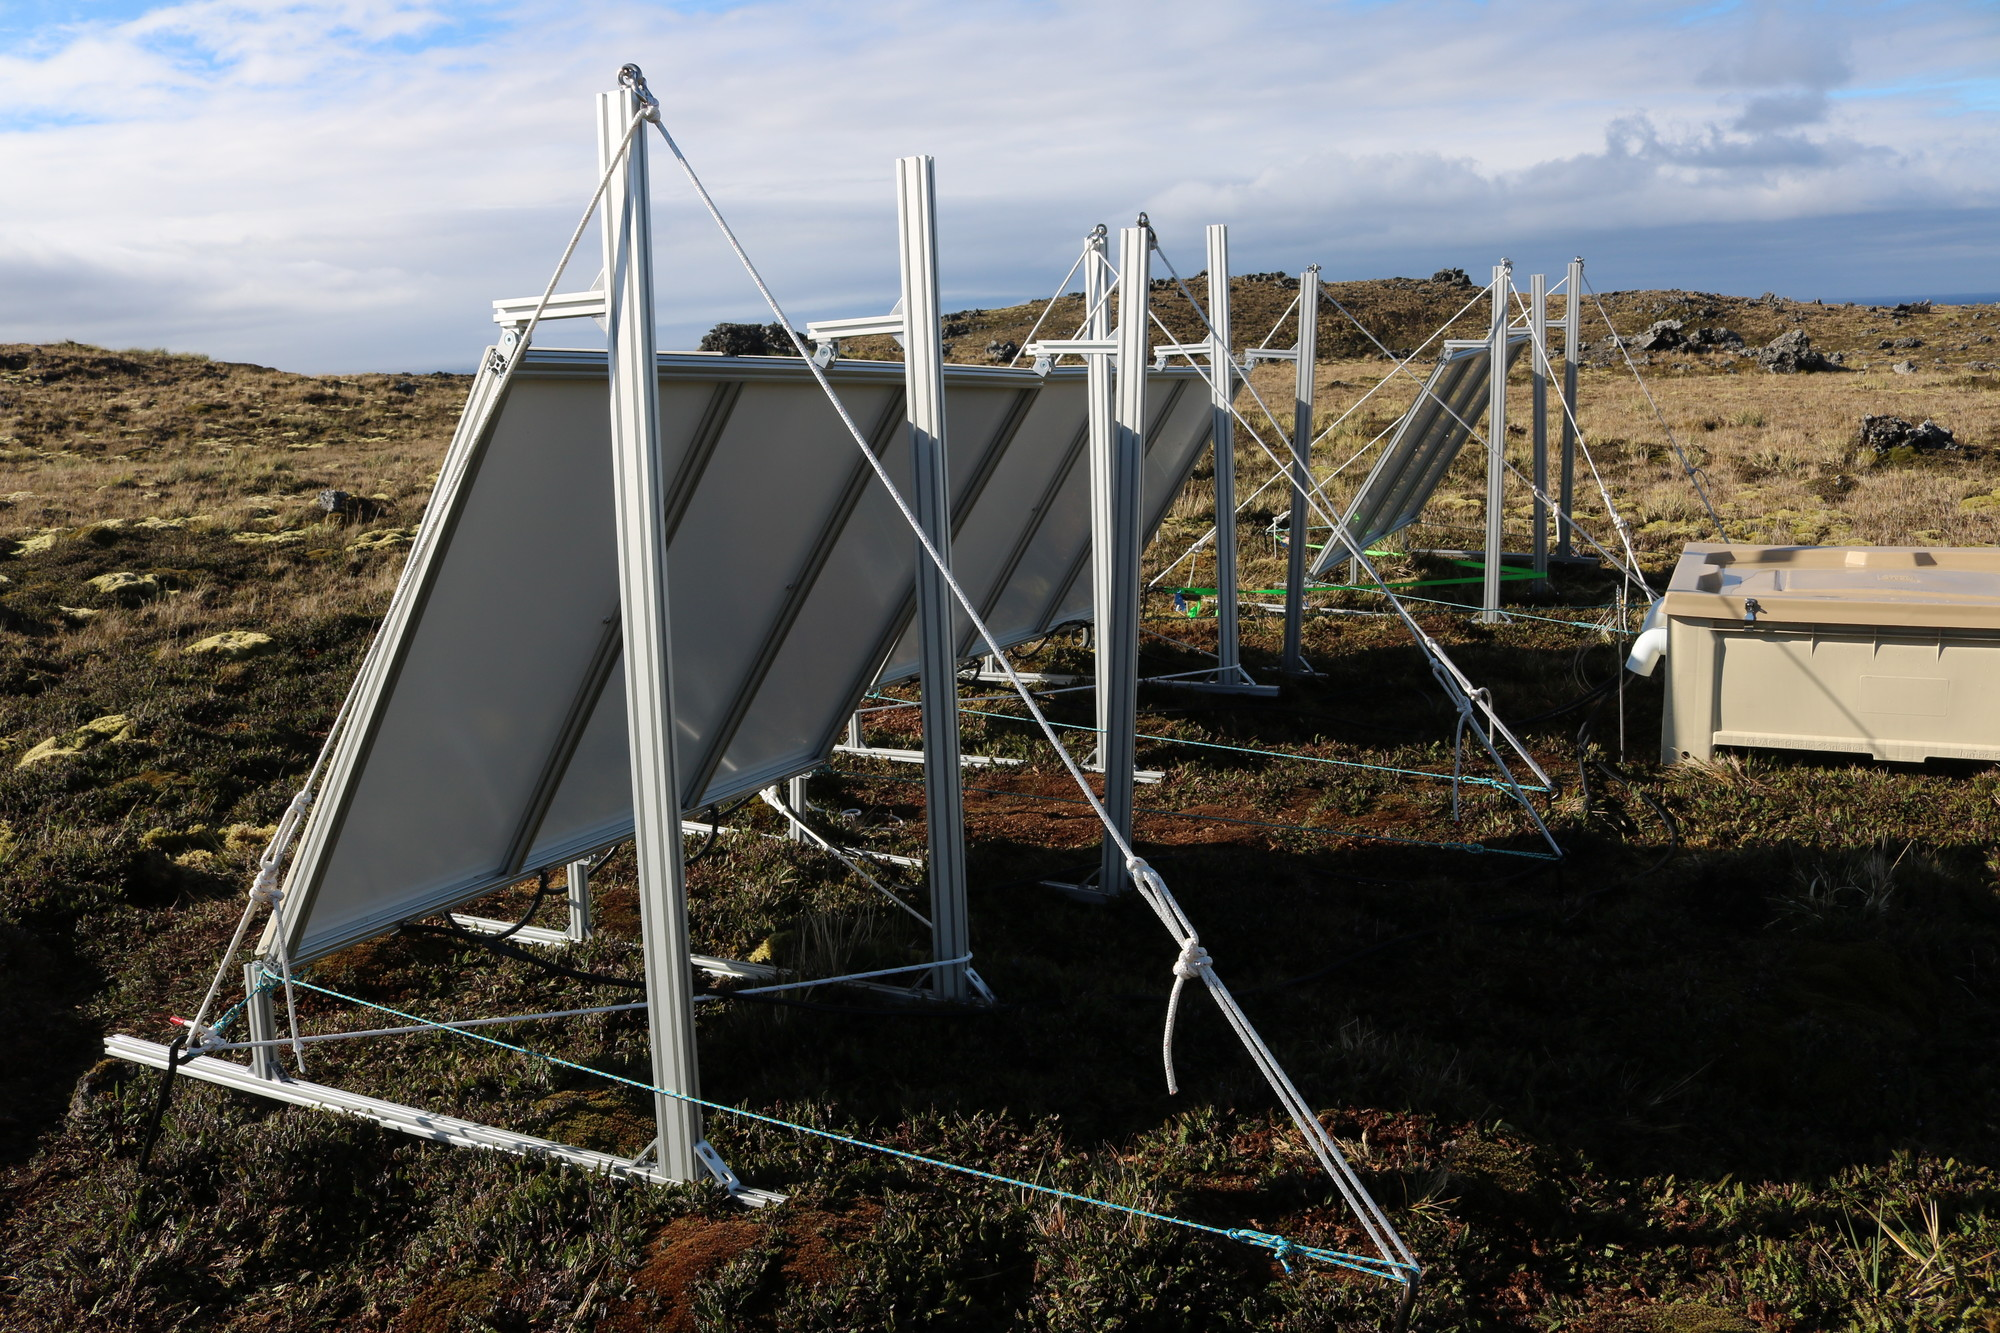
\includegraphics[width=\linewidth]{Figures/40916139043_f3d0c6b013_o} 
		\caption{} \label{Fig:40916139043_f3d0c6b013_o}
	\end{subfigure}
	\hfill
	\begin{subfigure}[t]{0.46\textwidth}
		\centering
		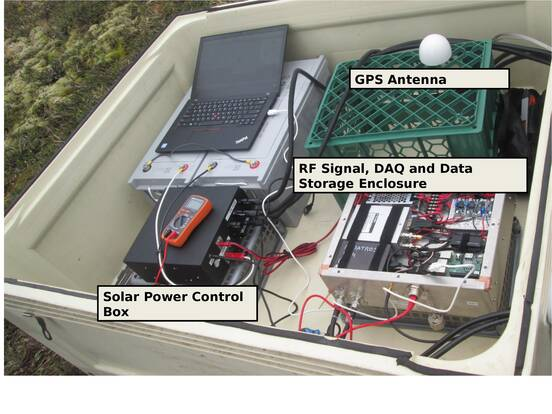
\includegraphics[width=\linewidth]{Figures/bin}
		\caption{} \label{Fig:bin}
	\end{subfigure}
	\caption{{\bf (a)} The three supporting structures for the nine solar panels mounted on a rigid metalized plastic panels. Behind the supporting structures is the plastic enclosure housing the readout electronics, two batteries, and the power control electronics. {\bf (b)} Interior of the  plastic enclosure housing the readout electronics, two batteries, GPS antenna, and the power control electronics} \label{Fig:power}
\end{figure}

The nine solar panels' supporting structures were specifically designed to manage the gale-force winds on Marion Island. However, it was challenging to install them as the volcanic ground minimizes the appropriate anchoring ability. With Marion being an environmentally protected base, there are additional limitations on the type of anchoring hardware that can be used. Wind power was one of the available options. Marion has an ornithology research group, and it is environmentally protected; wind power infrastructure was not going to be accepted as it was going to attract the birds. The material used for the three mounting structures was the t-slotted extruded aluminum framing. All joints were designed to be adjustable to accommodate the uneven terrain and allow varying incline angles. Each of the structures carries three solar panels mounted on a rigid metalized plastic panel. The structures are oriented due north and are designed to incline the solar panels at a relatively steep angle to perform efficiently under winter conditions. The three supporting structures with mounted solar panels are shown in Figure~\ref{Fig:40916139043_f3d0c6b013_o}. Behind the supporting structures is the plastic enclosure housing the readout electronics, two batteries, and the power control electronics shown in Figure~\ref{Fig:bin}. The plastic enclosure is a Mpact 528H, made of rugged weatherproof plastic, modified to include a hinged lid and cable feedthrough points.  The feedthrough points were stuffed with brass scouring pads and sealed with a metal mesh cloth to prevent mice from entering. Each group of solar panels mounted on three structures is connected in series.
The three groups' three connections are connected parallel to the Victron BlueSolar MPPT 150$\vert$35 charge controller, optimizing power transfer from the solar array when charging is required. Monitors charge level reducing output current when the battery bank is fully charged. An Arduino logs the data from the Victron charge controller to an SD card and switches power on and off to the readout electronics box. The on/off feature is compulsory to avert battery system damage from intense discharge. Typically, for lead-acid batteries, the battery should never be discharged down to \SI{0}{\percent} state of charge, and ideally (to preserve battery cycle life) never or seldom below \SI{50}{\percent}. The system also has a battery power conservation feature, which schedules observations for distinct periods, often during the night when ionospheric conditions are more favorable. For the time being, observations were continuously done while the system is in engineering mode, but this feature will be used in the future to keep the data volume manageable. The power logging and control system, the Victron charge controller, and an EMI filter are housed together in an aluminum box shown in Figure~\ref{Fig:power_box_interior}. The solar charge controller generates RF noise, which would likely cause interferences; hence, an EMI filter was designed to minimize conducted emissions on the solar charge controller's photovoltaic side. Figure~\ref{Fig:station} shows the complete installation of the first autonomous station. Thus far, the hydro shack installation was the first and only fully autonomous station deployed on the island. Additionally, baseband-ready readout boxes are used with the 2-element pathfinder at the \prizm\ site. The only missing aspect of Junior's setup is the power autonomy, but there is the capability to record baseband from both Junior's and hydro shack at the same time.

\begin{figure}
	\centering
	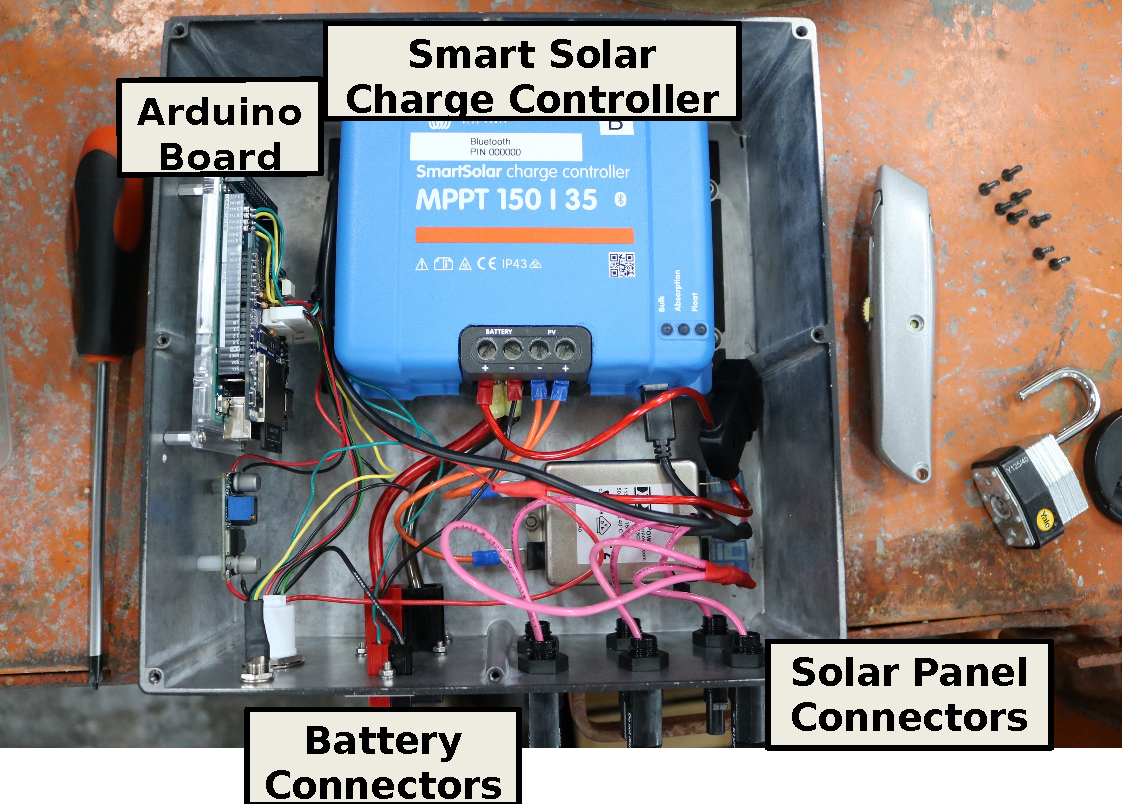
\includegraphics[width=\linewidth]{Figures/power_box_interior}
	\caption{The power logging and control system, the Victron charge controller, and an EMI filter are housed in an aluminum box.}
	\label{Fig:power_box_interior}
\end{figure}

\begin{figure}
	\centering
	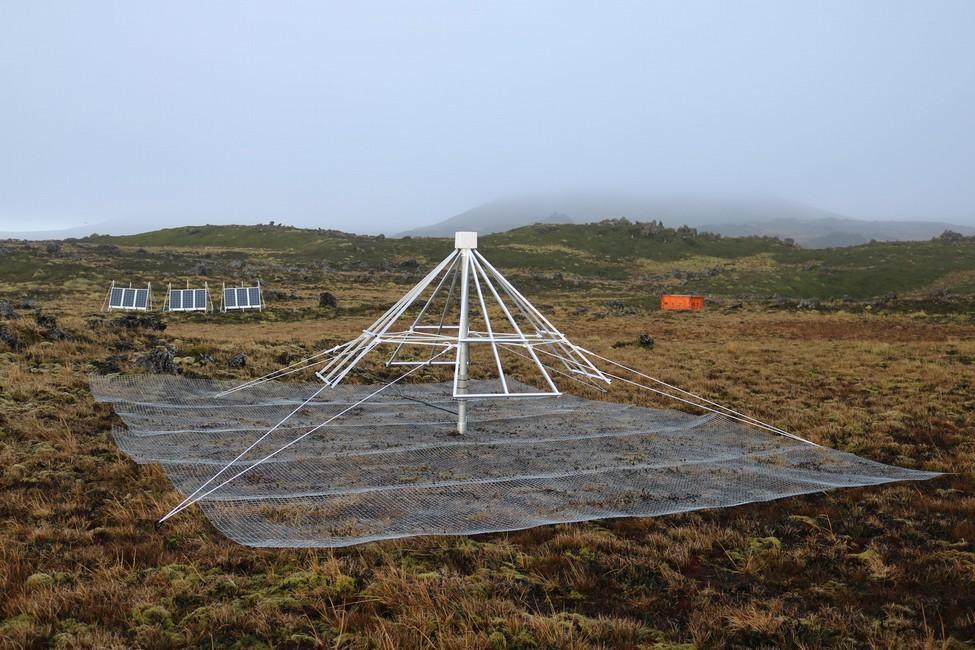
\includegraphics[width=\linewidth]{Figures/station}
	\caption{April 2019 deployment of the first \albatros\ autonomous station was a success. The mounted solar panels and the LWA antenna are visible. The hardware for the first autonomous station was enclosed in the orange container, and it was only present temporarily during the takeover period.}
	\label{Fig:station}
\end{figure}
